% =============================================================================
% Chapter 14 — The Quantized Bet: EXL3 on GB10
% =============================================================================
\chapter{The Quantized Bet: EXL3 on GB10}
\label{ch:quantized-bet}

On the same serving stack, a community contributor's 4-bit quant of
GLM-5.3-Flash scores a mean KLD of 0.024555 nats against the full-precision
teacher; the official FP8 release scores 0.024629 --- a statistical tie, at
54\,\% of the bytes (176 vs.\ 328\,GB). That number is the pivot on which
the second half of this book turns. If four bits per weight can preserve the
teacher distribution as well as the official release does, a frontier-class
model fits in roughly half the memory --- on hardware where every byte of
LPDDR5X bandwidth is the throughput budget.

Part~I told the story of one bet: serve DeepSeek-V4-Flash on 2$\times$~DGX
Spark in the checkpoint's own native NVFP4 weights, and spend the engineering
budget on the scheduler, the drafter, and the fabric. Part~II follows the
sibling repository, \code{GLM-5.3-Flash-EXL3-2x-DGX-Sparks}, which takes the
same two GB10 machines, the same vLLM TP=2 topology over a ConnectX-7 cable,
and makes the opposite bet: a 320B-class MoE quantized by a community
contributor to 4 bits per weight in a trellis format the serving stack has
never heard of. Everything Part~I established --- the hardware envelope
(\Cref{ch:problem}), MLA anatomy (\Cref{ch:model}), patch discipline
(\Cref{ch:patches}), measurement culture (\Cref{ch:measurement}) --- carries
over; these chapters cover only what is new.

And what is new is substantial, because the tie is not free. A native
checkpoint arrives blessed; a community quant arrives owing proof. The
quantized bet forces four pieces of engineering that the native-precision
recipe never needed: a provenance chain that treats weight availability as an
operational dependency; a quantitative quality case (because a 4-bit quant
must \emph{prove} it is not a lobotomy); an attention-geometry overlay,
because stock vLLM cannot even load this model's KV layout on this silicon;
and a complete vLLM quantization backend written from scratch, including
purpose-built CUDA kernels that bought a measured 20\,\% of prefill.

Any deployment that steps off the vendor's paved path --- a community quant,
an unusual attention geometry, a format the engine's kernel zoo does not
instantiate --- inherits some subset of the same obligations. This chapter
walks what each looks like engineered rather than improvised:
pinned mirrors instead of hopeful URLs, KLD panels instead of adjectives,
exactness arguments instead of new kernels, and a backend whose core
promises are enforced with hard errors.

\section{The recipe on one page}
\label{sec:qbet-recipe}

The repository serves \code{zai-org/GLM-5.3-Flash} --- a 320B-class mixture-of-experts
with 288 routed experts, hybrid KDA linear attention plus NoPE sparse MLA ---
as \textbf{brandonmusic's TR3 4-bpw EXL3 quant}: uniform-K4 EXL3/TR3
routed-experts trellis, roughly 164\,GiB across \textbf{120 safetensors
shards}. Only the routed experts are quantized; dense layers, shared experts,
attention, embeddings, and \code{lm_head} stay native BF16.

The deployment mirrors Part~I's shape: vLLM's \code{mp} executor with
\code{--tensor-parallel-size 2} across two nodes joined by the CX7 QSFP cable
(RoCEv2), the OpenAI-compatible API on port \code{:8888} on the head node,
served model id \code{GLM-5.3-Flash-EXL3}, and a full
\textbf{1M-token context} (\envvar{MAX_MODEL_LEN=1000000}) with prefix
caching and CUDA graphs on. Speculative decoding runs the DFlash2 drafter at
$k{=}7$ --- the next chapter's subject --- with MTP $k{=}2$ as the rollback.

Because the weights are a third party's quant rather than the vendor's own,
the recipe must carry its own quality evidence (\Cref{sec:qbet-quality}),
its own kernels (\Cref{sec:qbet-e2}), and, less obviously, its own insurance
against the upstream artifact disappearing (\Cref{sec:qbet-provenance}).

\section{Provenance as engineering}
\label{sec:qbet-provenance}

A native-precision recipe points at a vendor repository and moves on. A
community-quant recipe has a supply chain, and this repository engineers it
explicitly as a three-link chain, each link documented in the README:

\begin{enumerate}
  \item \code{zai-org/GLM-5.3-Flash} --- the upstream base model.
  \item \code{brandonmusic/GLM-5.3-Flash-tr3-4bpw} --- the EXL3/TR3 quant,
    pinned at Hub snapshot \code{5ab363a8}.
  \item \code{Mia-AiLab/GLM-5.3-Flash-EXL3-TR3-4bpw} --- a
    \emph{byte-identical public mirror} of that snapshot, pinned to Hub
    commit \code{25a44fdbf16862a46b7cc9921142c6c81350af2f}.
\end{enumerate}

The mirror exists for one reason, stated in the commit that created it: ``so
new clones survive an upstream rename.'' Hugging Face repository ids are
mutable --- accounts rename, quants get reorganized --- and a serving recipe
whose launcher hard-codes someone else's namespace inherits that fragility.
The launcher therefore points \envvar{MODEL} at the lab's own mirror and
keeps \envvar{MODEL_FALLBACK=brandonmusic/GLM-5.3-Flash-tr3-4bpw} as the
escape hatch, used if the mirror 404s or turns out incomplete.

\begin{figure}[htbp]
\centering
\begin{tikzpicture}[node distance=7mm and 10mm]
  \node[hbnode, minimum width=62mm] (up)
    {\textbf{zai-org/GLM-5.3-Flash}\\upstream base model (NoPE MLA)};
  \node[hbbox, below=of up, minimum width=62mm] (quant)
    {\textbf{brandonmusic/GLM-5.3-Flash-tr3-4bpw}\\EXL3/TR3 4\,bpw quant --- snapshot 5ab363a8\\$\approx$164\,GiB, 120 shards};
  \node[hbgpu, below=of quant, minimum width=62mm] (mirror)
    {\textbf{Mia-AiLab/GLM-5.3-Flash-EXL3-TR3-4bpw}\\byte-identical mirror, pinned 25a44fdb\ldots};
  \draw[hbflow] (up) -- node[hblabel, right=1mm] {quantize (community)} (quant);
  \draw[hbflow] (quant) -- node[hblabel, right=1mm] {mirror (survive Hub renames)} (mirror);
  % launcher side
  \node[hbbox, right=16mm of mirror, minimum width=34mm] (launcher)
    {launcher\\MODEL = mirror};
  \node[hbpatch, above=of launcher, minimum width=34mm] (gate)
    {gate: 120 shards\\present?};
  \draw[hbflow] (launcher) -- (gate);
  \draw[hbok] (gate.west) to[out=180,in=0]
    node[hblabel, above, sloped] {$\geq$120: serve} (mirror.east);
  \draw[hbfail] (gate.north) to[out=90,in=0]
    node[hblabel, above, sloped] {404 / $<$120: fallback} (quant.east);
\end{tikzpicture}
\caption{The weight provenance chain. The recipe serves from a byte-identical
mirror of brandonmusic's pinned snapshot so that an upstream Hub rename
cannot strand new clones; the launcher falls back to the original repository
if the mirror is missing or holds fewer than the expected 120 shards.}
\label{fig:qbet-provenance}
\end{figure}

The 120-shard count is not trivia --- it is the completeness invariant
(\envvar{EXPECTED_SHARDS=120}) enforced at three points. The download step
dies with ``download finished with N / 120 shards'' if either source
delivered a partial tree. Before downloading at all,
\code{adopt_complete_weights} checks whether the primary cache directory
already holds at least 120 shards and, failing that, whether the
\emph{fallback} cache does --- in which case it silently switches
\code{MODEL_PATH} to the brandonmusic folder rather than pulling a second
164\,GiB copy of bytes it already has.

The worker sync is guarded by a revision marker keyed on the snapshot
commit. A model or revision switch re-syncs automatically; an unchanged tree
skips the full size-and-mtime verification walk over 120 shards on both
ends. Downloads pin
\code{--revision} only for the primary repo id; the mirror's pinned commit is
what makes ``byte-identical'' an enforceable claim rather than a hope.

None of this is peculiar to community quants. Any serve that resolves its
weights by name against a mutable registry carries an unpinned dependency in
its boot path, and the failure arrives as a 404 on a fresh clone months
later rather than as a change someone reviewed.

\section{The quality case}
\label{sec:qbet-quality}

The mirror and its shard gates guarantee that the bytes arrive; they say
nothing about what the bytes are worth. A 4-bit community quant of a
frontier model invites an obvious objection:
how much of the model survived? The repository answers with numbers rather than
adjectives, citing malaiwah's independent teacher-logit KLD panel (published
in discussion \#1 on brandonmusic's Hub repository): KLD(teacher\,$\|$\,model)
over five cold runs and 25 sealed windows totaling 51{,}175 positions.
\Cref{tab:qbet-kld} reproduces it.

\begin{table}[htbp]
\centering\small
\caption{Independent KLD panel (malaiwah, brandonmusic Hub discussion \#1):
mean KLD(teacher\,$\|$\,model) in nats, five cold runs, 25 sealed windows,
51{,}175 positions. Lower is better; the panel scores the weights, not the
GB10 overlay.}
\label{tab:qbet-kld}
\begin{tabular}{lrr}
\toprule
Model & Mean KLD (nats) & Size \\
\midrule
TR3 K6 (6\,bpw) & 0.013723 & 254\,GB \\
Official FP8 (cross-stack) & 0.020615 & 328\,GB \\
\textbf{This checkpoint --- EXL3 4\,bpw} & \textbf{0.024555} & \textbf{176\,GB} \\
Official FP8 (brandonmusic stack, v44) & 0.024629 & 328\,GB \\
NVFP4 (brandonmusic stack, v44) & 0.060535 & $\approx$180\,GB \\
\bottomrule
\end{tabular}
\end{table}

\begin{hbnote}
KLD(teacher\,$\|$\,model) measures, position by position, how far the
quantized model's next-token distribution diverges from the full-precision
teacher's --- zero would mean the quant reproduces the teacher's output
distribution exactly. It is a stricter instrument than task benchmarks:
a benchmark can hide distributional damage behind ties and sampling noise,
while KLD integrates every position of every window. The ``sealed windows''
and cold runs matter for the same reason the cold-prefill protocol salts its
prompts --- an evaluation the evaluated party cannot overfit.
\end{hbnote}

The headline is the middle two rows: on the same serving stack, the 4\,bpw
EXL3 quant scores 0.024555 against the official FP8's 0.024629 --- a
statistical tie --- \textbf{at 54\,\% of the bytes} (176 vs.\ 328\,GB). That
is the entire quantized bet in one line: EXL3's trellis coding preserves the
teacher distribution as well as FP8 does, in half the memory, on a machine
where memory traffic is the throughput ceiling.

The bottom row is the
counter-example that hardens the recipe's sharpest rule: an NVFP4 quant of
the same model, at a similar size to the EXL3 build, scores 0.060535 ---
roughly $2.5\times$ worse KLD. What was the native, correct choice for
DeepSeek-V4-Flash in Part~I is a measurably damaging choice for this
checkpoint.

\begin{hbwarning}
Never pass \code{--moe-backend marlin} to this recipe, and never substitute
NVFP4 weights. The invariant appears verbatim at the top of both
\repofile{start.sh} and the Dockerfile: ``EXL3, not NVFP4. Do not pass
--moe-backend marlin.'' The marlin flag is the NVFP4 FLASHINFER\_CUTLASS
workaround --- the wrong backend for an EXL3 checkpoint. The KLD panel
(\Cref{tab:qbet-kld}) is the quantitative reason the NVFP4 route is banned
outright: $2.5\times$ the divergence at a comparable byte count. A related trap:
the Hub card on brandonmusic's repository describes an SM120 image
(TP2/EP2/DCP2 with calibrated NVFP4 MLA KV) that is \emph{not} this overlay.
This recipe is EXL3 weights plus \code{fp8_ds_mla} target KV on GB10
(SM121); conflating the two images is a documented failure mode.
\end{hbwarning}

\section{Teaching stock vLLM a geometry it lacks}
\label{sec:qbet-geometry}

Quality settled, there is a harder problem: stock vLLM cannot serve this
model on this silicon at all. The pinned base image
(\code{vllm/vllm-openai:glm53-flash-arm64-cu130}, by digest) loads the
checkpoint and dies on the first forward pass with
\code{pe_dim must be 64 for fp8_ds_mla}. The 88-line header comment of the
repository's Dockerfile is the design document for why.

GLM-5.3-Flash is \emph{NoPE MLA}: \code{qk_rope_head_dim=0} and
\code{kv_lora_rank=512}, so the attention latent is 512 dimensions with no
RoPE component at all (contrast \Cref{ch:model}'s DeepSeek MLA, which
carries a 64-dim RoPE block).

On SM12x the only sparse-MLA backend is
\code{FLASHINFER_MLA_SPARSE_SM120}, and its kernels are instantiated for
fixed geometries: the DSV3\_2 and GLM\_NSA model types at
$d_{qk}=576$ with a packed 656\,B/token record, and DSV4 at
$d_{qke}=512$ with a 584\,B record but a top-$k$ set that stops at 1024.
GLM-5.3-Flash needs $d_{qk}=512$ with \code{index_topk=2048} --- in the
Dockerfile's words, ``which no kernel instantiates.'' No amount of
configuration reaches a kernel that does not exist.

The two subsections that follow are the overlay's answer, and neither of
them is a kernel. One reshapes the checkpoint's request until an
already-compiled kernel accepts it; the other trims that request to a width
fixed at compile time --- both paying a bounded, quantified price to avoid
owning new CUDA.

\subsection{The zero-pad: exactness by arithmetic}

The overlay's fix is disarmingly simple: \textbf{zero-pad the 512-dim latent
into the 576-wide GLM\_NSA geometry}. The packed record becomes 512 bytes of
NoPE latent, 16 bytes of scales, and a 128-byte RoPE region that is all
zeros; queries are padded to 576 the same way. The correctness argument is
one sentence of linear algebra: a zero RoPE block contributes nothing to the
QK dot product, so every attention score is unchanged, softmax is unchanged,
and the value is read from the 512-dim NoPE region ($d_v=512$) --- the
result is \emph{mathematically exact}, not approximate. The cost is pure
storage: 656\,B/token instead of the $\approx$528\,B a native $d_{qk}=512$
record would take, about 24\,\% more sparse-attention KV across the 11 DSA
layers --- and \emph{zero} kernel work. On a machine where writing a new
sparse-MLA kernel means owning it forever, buying exactness with a quarter
more KV on one cache family is an excellent trade.

\begin{figure}[htbp]
\centering
\adjustbox{max width=\textwidth}{%
\begin{tikzpicture}
  % checkpoint latent
  \node[hbtitle, anchor=west] at (0,3.1) {Checkpoint: NoPE MLA latent (no kernel exists at $d_{qk}=512$, topk 2048)};
  \draw[thick, fill=ice, draw=teal] (0,2.0) rectangle (7.6,2.7);
  \node[font=\small] at (3.8,2.35) {512-dim NoPE latent};
  \node[hblabel, anchor=west] at (8.0,2.35) {qk\_rope\_head\_dim = 0};
  % packed record
  \node[hbtitle, anchor=west] at (0,1.3) {Overlay: packed into FlashInfer's GLM\_NSA 656\,B/token record ($d_{qk}=576$)};
  \draw[thick, fill=brandgreen!12, draw=brandgreen!70!black] (0,0.2) rectangle (7.6,0.9);
  \node[font=\small] at (3.8,0.55) {512\,B NoPE (fp8)};
  \draw[thick, fill=ice, draw=teal] (7.6,0.2) rectangle (8.6,0.9);
  \node[font=\scriptsize] at (8.1,0.55) {16\,B};
  \draw[thick, fill=lightgray!45, draw=brandgray] (8.6,0.2) rectangle (11.4,0.9);
  \node[font=\small] at (10.0,0.55) {128\,B RoPE = 0};
  \node[hblabel, anchor=north] at (8.1,0.1) {scales};
  \node[hblabel, anchor=north west] at (8.6,0.1)
    {zero block: adds nothing to $q\cdot k$ --- exact};
  \draw[hbflow, rounded corners=3pt]
    (0,2.35) -- (-0.85,2.35) -- (-0.85,0.55) -- (0,0.55);
  % cost note
  \node[hblabel, anchor=west] at (0,-0.75)
    {cost: 656\,B/token vs $\approx$528\,B native ($\approx$24\,\% more DSA KV over 11 layers); kernel work: none};
\end{tikzpicture}}
\caption{Fix 1 of the NoPE overlay: the 512-dim latent is zero-padded into
FlashInfer's 576-wide GLM\_NSA packed record. The zero RoPE block cannot
change any QK dot product, so the attention result is mathematically exact
--- the overlay buys an existing kernel with $\approx$24\,\% more
sparse-attention KV instead of writing a new one.}
\label{fig:qbet-zeropad}
\end{figure}

\subsection{The 2051-candidate squeeze}

A subtler constraint hides in the same kernel family: the sparse top-$k$
width is a compile-time \emph{template parameter}, and the SM120 prefill
kernel rejects any \code{topk != 2048}. But GLM's sparse indexer emits up to
\textbf{2051} candidates --- 512 pools $\times$ 4 tokens each, plus up to 3
tail tokens that have not yet closed a pool. Three candidates too many, and
the width cannot be negotiated at runtime.

The overlay's resolution shows exactly where the engineering judgment lives:
\textbf{drop the lowest-ranked selected pool, keep the tail}. Expanding 511
pools yields 2044 tokens; adding the 3 tail tokens gives 2047 candidates in
the 2048-wide buffer. What is sacrificed is 4 of 2048 candidate tokens ---
0.2\,\% --- and specifically the \emph{last} ones in top-$k$ rank order, the
pool the indexer itself scored least relevant. What is preserved is the
recent causal tail, and the asymmetry is the whole argument: in a causal
model the most recent tokens carry the highest attention weight. And unlike
a mid-context pool --- which, if dropped, could in principle be re-selected
at the next step --- the tail tokens are not members of any closed pool yet,
so discarding them would lose information \emph{that no pool expansion can
ever recover}. The lowest-ranked pool is expendable by the indexer's own
ranking; the tail is unrecoverable by construction. (\code{select_k} stays
512, keeping the fused top-$k$ fast path intact.)
\Cref{fig:qbet-squeeze} draws the trade.

\begin{figure}[htbp]
\centering
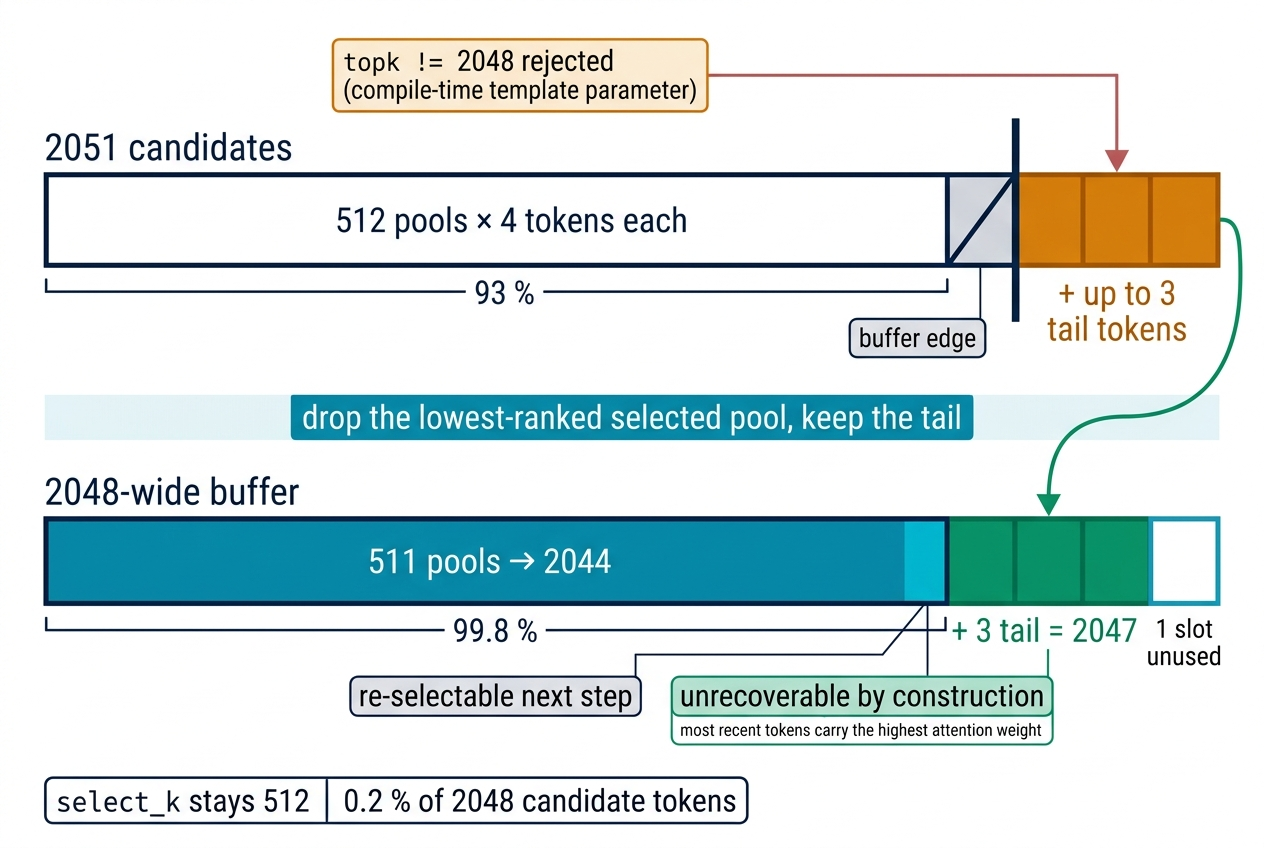
\includegraphics[width=\textwidth]{figures/ch14-candidate-squeeze.png}
\caption{Fix 2 of the NoPE overlay. The sparse indexer emits up to 2051
candidates --- 512 pools of 4 tokens, plus up to 3 tail tokens that have not
yet closed a pool --- while the SM120 prefill kernel's top-$k$ width is a
compile-time template parameter fixed at 2048. Dropping the lowest-ranked
pool costs 4 candidate tokens (0.2\,\%) that the indexer itself scored least
relevant and that a later step could in principle re-select; truncating the recent tail
instead would discard the highest-weighted tokens in a causal model, and no
pool expansion could ever recover them.}
\label{fig:qbet-squeeze}
\end{figure}

\section{A quantization backend from scratch}
\label{sec:qbet-exl3py}

With the KV geometry solved, the weights still need kernels. A quantization
backend in vLLM is best read as a claim of ownership: the registered module
takes responsibility for how the layers it claims are stored, sharded, and
multiplied, and every layer it does not claim falls through to the engine's
stock paths.
\repofile{overlay/exl3.py} (1{,}623 lines) is a complete vLLM quantization
backend --- not a patch of an existing one, but a new module registered with
\code{@register_quantization_config("exl3")} and dropped into the image's
quantization package (an 11-line companion patch adds \code{"exl3"} to
\code{ModelConfig}'s override list so vLLM will claim the checkpoint).
Its scope is deliberately narrow: \code{quant_method=exl3, codebook=mcg,
scope=glm53_routed_experts_only}. Only the routed experts run quantized;
everything else takes vLLM's stock \code{UnquantizedLinearMethod}.

Three design decisions define the file, and each is best read from the
failure it prevents. First, a packed-ABI disagreement between the checkpoint
and the kernels would be silent corruption --- so \textbf{the checkpoint ABI
is asserted, not assumed}. Each expert matrix ships as \code{trellis}
(packed int16 codes), \code{suh}/\code{svh} (fp16 input/output Hadamard
sign-scale vectors), and an int32 \code{mcg} marker whose value must be the
MCG multiplier \code{0xCBAC1FED};\footnote{Stored, in int32's signed
rendering, as $-877912083$.} \code{process_weights_after_loading} checks
that marker on \emph{every expert} and raises a hard \code{RuntimeError} on
mismatch --- corruption, never a warning. The exllamav3 dependency is pinned
to the same standard --- commit \code{c5d9c657}, version 0.0.43, the pin that
exposes the fused \code{exl3_moe} entry points.

Second, without the method actually claiming the layers, vLLM's default
loader would quietly expand every routed expert to BF16 --- tripling the
routed-expert footprint and OOMing the machine --- so \textbf{experts never
materialize in BF16}. \code{create_weights} registers only the packed
parameters --- the trellis tensors, Hadamard vectors, and markers for the
gate/up and down projections --- and then \emph{raises} if the dense buffers
\code{w13_weight} or \code{w2_weight} exist on the layer. That negative
promise, not the \code{"exl3"} registration itself, is what makes 164\,GiB
fit on two unified-memory GB10 nodes. TP=2 sharding follows the usual MoE
convention (gate/up column-wise, down row-wise, one all-reduce per layer),
with \code{_narrow_tp} raising on any non-divisible dimension.

Third, executing \code{exllamav3/__init__.py} would drag FlashAttention and
serving extras absent from this image into the boot --- so \textbf{the
dependency is imported surgically}. The backend needs exactly one class,
\code{LinearEXL3}, and \code{_install_exllamav3_namespace()} fabricates just
enough stub modules for
\code{exllamav3.modules.quant.exl3.LinearEXL3} to import cleanly through a
skeleton of its own package.\footnote{Stub \code{types.ModuleType} entries
for \code{exllamav3}, \code{exllamav3.modules}, and \code{exllamav3.model},
plus a fake \code{Config} class, leaving \code{.ext}, \code{.util}, and
\code{.modules.quant} real.} It is the same patch-discipline instinct as
\Cref{ch:patches}, applied to Python's import system: take exactly what you
need, and make every assumption about the rest explicit.

At runtime the fused path (\envvar{EXL3_FUSED_MOE=1}, the default) builds
GPU pointer tables for all nine tensor families (gate/up/down $\times$
trellis/suh/svh) and serves each decode layer with a single
\code{exllamav3_ext.exl3_moe} launch. The shared temp buffers are sized to
\envvar{EXL3_TEMP_ROWS_FUSED} rows per expert --- default 128. That number
is a measured boundary, not a guess: it defines who counts as a ``fat''
expert, and the next section is about what happens to them.

\section{The fat-expert tier ladder}
\label{sec:qbet-tiers}

Decode batches are small; the fused kernel's 128-row-per-expert budget covers
them in one graph-safe launch. Prefill is the opposite regime: at chunk size
2048, top-8 routing over 288 experts means essentially \emph{every} expert
activates, and the hottest experts see far more than 128 rows. (The P0
profile in \Cref{sec:qbet-warstory} measured 98.6\,\% of MoE layers hitting
the fat path at $\approx$920 rows for the hottest expert.) The fused kernel
simply skips any expert whose token count exceeds the temp rows, so fat
experts need a second pass --- and the backend offers four implementations of
that pass, arranged as a strict ladder resolved once, at weight load:

\begin{description}
  \item[kernel (E2)] direct trellis GEMMs --- \code{ext.exl3_fat_gemm} for
    the stacked gate+up projection and \code{ext.exl3_fat_gemm_scatter} for
    the down projection with fused routing (\Cref{sec:qbet-e2}).
  \item[batched (E1)] persistent scratch buffers; routing counts staged
    device-to-host on a side CUDA stream while the thin-expert launch
    proceeds; gate and up trellises stacked into one GEMM behind a single
    input Hadamard --- legal only because the checkpoint shares its input
    sign-scale vector (SUH) between gate and up, a fact \emph{verified at
    load} by \code{torch.equal} on the two halves of \code{w13_suh}.
    Without the E2 kernel this tier reconstructs fp16 weights into scratch
    and runs \code{ext.hgemm} plus an output-Hadamard pass.
  \item[sorted] reuses the already-sorted token/weight buffers so one
    \code{counts.tolist()} replaces all per-expert host syncs; contiguous
    slices are views.
  \item[legacy] the original Python loop over fat experts: per-expert
    \code{unique().tolist()}, \code{nonzero()}, three \code{LinearEXL3}
    forwards, SwiGLU, \code{index_add_} scatter --- many host syncs per
    layer.
\end{description}

Each tier's env knob implies the ones below it
(\envvar{EXL3_FAT_KERNEL=1}, the shipped default, implies batched and
sorted). The resolution logic is where the repository's failure philosophy
crystallizes:

\begin{lstlisting}[language=Python]
# resolve_exl3_fat_tier -- runs once, at weight load
if EXL3_FAT_KERNEL:
    if not (sym_exl3_fat_gemm and sym_exl3_fat_gemm_scatter):
        raise RuntimeError(...)   # "unset EXL3_FAT_KERNEL or serve an E2 image"
    if not shared_suh:
        tier, reason = "sorted", "shared_suh_absent"   # recorded, legitimate
    else:
        tier = "kernel"
elif EXL3_FAT_BATCHED: ...        # same shared-SUH gate
elif EXL3_FAT_SORTED:  tier = "sorted"
else:                  tier = "legacy"
\end{lstlisting}

Two outcomes that look superficially similar are treated in opposite ways.
An image whose extension lacks the E2 symbols while
\envvar{EXL3_FAT_KERNEL=1} is a \emph{configuration lie} --- the operator
asked for a kernel that does not exist. The backend fails closed at boot
with a \code{RuntimeError} naming the missing symbol, before the server can
take a request. A checkpoint that does not share SUH between gate and up
is merely a \emph{different checkpoint}: the stacked-GEMM optimization is
unavailable, so the tier degrades to \code{sorted} with the recorded reason
\code{shared_suh_absent} --- slower, correct, and visible in the diagnostics.

\begin{hblesson}
Degradation is legitimate; mismatch is fatal. A system may run slower than
configured when the \emph{data} does not support an optimization, provided
it records why --- but it must never run at all when the \emph{deployment}
contradicts its configuration. The boundary is who is wrong: if the
checkpoint lacks a property, the ladder steps down and says so; if the image
lacks a symbol the operator explicitly enabled, silently stepping down would
convert a build mistake into weeks of unexplained slow prefill. The GLM
recipe repository learned this concretely: before the recipe-stamp rebuild
mechanism landed in PR \ghissue{77}, \envvar{EXL3_FAT_KERNEL=1} on the older
public GHCR image had been a silent no-op --- exactly the failure mode the
load-time \code{RuntimeError} now makes impossible.
\end{hblesson}

\begin{figure}[htbp]
\centering
\begin{tikzpicture}[node distance=5mm and 12mm]
  \node[hbtitle] (t) {Fat-expert tier ladder --- resolved once at weight load};
  \node[hbgpu, below=4mm of t, minimum width=58mm] (k)
    {\textbf{kernel (E2)} --- direct trellis GEMMs\\exl3\_fat\_gemm + \_scatter};
  \node[hbbox, below=of k, minimum width=58mm] (b)
    {\textbf{batched (E1)} --- persistent scratch,\\stacked gate+up, side-stream D2H counts};
  \node[hbnode, below=of b, minimum width=58mm] (s)
    {\textbf{sorted} --- one counts.tolist(),\\contiguous slice views};
  \node[hbfaint, below=of s, minimum width=58mm] (l)
    {\textbf{legacy} --- python loop,\\per-expert host syncs};
  \draw[hbarrow] (k) -- (b);
  \draw[hbarrow] (b) -- (s);
  \draw[hbarrow] (s) -- (l);
  % gates
  \node[hbwarn, right=of k, minimum width=44mm] (boom)
    {EXL3\_FAT\_KERNEL=1,\\symbols missing:\\\textbf{RuntimeError at load}};
  \draw[hbfail] (k.east) -- (boom.west);
  \node[hbpatch, right=of b, minimum width=44mm] (suh)
    {shared gate/up SUH absent:\\degrade to \emph{sorted},\\reason recorded};
  \draw[hbarrow] (suh.west) -- (b.east);
  \draw[hbarrow] (suh.south) to[out=-90,in=0] (s.east);
  \node[hblabel, below=2mm of l, align=center]
    {each knob implies the tiers below it; shipped default EXL3\_FAT\_KERNEL=1};
\end{tikzpicture}
\caption{The fat-expert tier ladder in \code{overlay/exl3.py}. The highest
enabled tier wins, resolved at weight load. A missing kernel symbol under
\code{EXL3_FAT_KERNEL=1} is a deployment mismatch and fails the boot; a
checkpoint without shared SUH is a legitimate degradation to the sorted tier
with a recorded reason.}
\label{fig:qbet-ladder}
\end{figure}

\section{The road to PR~77}
\label{sec:qbet-warstory}

The top rung of that ladder --- the E2 kernel --- did not begin as a kernel
project. It began as a profiling assignment --- and two published failures.

\begin{hbwarstory}
The prefill investigation (\repofile{docs/improve-prefill.md}, 2026-08-29)
opened with a roofline that pointed at weight streaming: at MNBT 1024,
routed-expert traffic alone was estimated at $\ge$330\,ms of a
1.05--1.10\,s engine step, memory-bound at that chunk size. The plan's step
P0 was ``profile first --- decides everything,'' and it did: the torch
profiler attributed \textbf{63\,\%} of the 1.08\,s step (623\,ms) to
\code{moe_forward_shared}, but split it damningly. The fused
\code{exl3_moe} kernel itself was only 134\,ms; 64\,ms went to
\code{LinearEXL3} weight reconstruction and 52\,ms to the
\code{index_add_} fat scatter. On the CPU side, a single
\code{.nonzero().tolist()} host sync in the fat fallback burned
\textbf{29\,\% of CPU} (1.45\,s in a 3-step capture). The suspects the
roofline could not rank turned out to be innocent: KDA measured only
$\approx$6\,\% and the sparse indexer $\approx$4\,\%, both flat from 16k to
100k context. The bottleneck was not the quantized GEMM --- it was
everything wrapped \emph{around} it for fat experts.

The two obvious fixes both failed, and the repository published the failures with
the same prominence as the wins. P2a (GPU 128-row tiling of fat experts):
$-61$\,\% at 8k, reverted, kept behind \envvar{EXL3_MOE_ROW_TILE=0} as an
escape hatch. P2b (raising \envvar{EXL3_TEMP_ROWS_FUSED} to 1024 so the
fused kernel swallowed fat experts in one launch): slower on \emph{every}
rung, worst $-24$\,\% at 100k --- the trellis kernel does not sustain large
per-expert M. What survived was the modest MNBT 2048 keep ($+16$\,\% at 8k)
and an honest sentence: the aspirational ceiling was not reached ``so larger
chunks could not drop the LinearEXL3 fat tax.'' Three days later PR
\ghissue{77} removed the fat tax properly --- with a kernel shaped by
exactly what P0 had measured: no reconstruction, no separate Hadamard pass,
no host-syncing scatter. The failed experiments were not wasted work; they
were the specification. The same plan also priced what was never built: its
P7 entry costed UMA KV stage-out/stage-in for evicted sessions at
$\sim$790\,MB $\approx$ 4\,ms against $\sim$105\,s of recompute --- ``the
cheapest prefill speedup in the list.'' It remains unbuilt: the
investigation stopped after P2, and P3--P8 were never started.
\end{hbwarstory}

The arc is Part~I's measurement discipline (\Cref{ch:measurement},
\Cref{ch:perf}) replayed in a new repository: profile before touching anything,
publish reverts next to keeps, and let the profile --- not the roofline ---
pick what gets built. \Cref{fig:qbet-p0} collects what P0 measured beside
what each measurement eventually bought.

\begin{figure}[htbp]
\centering
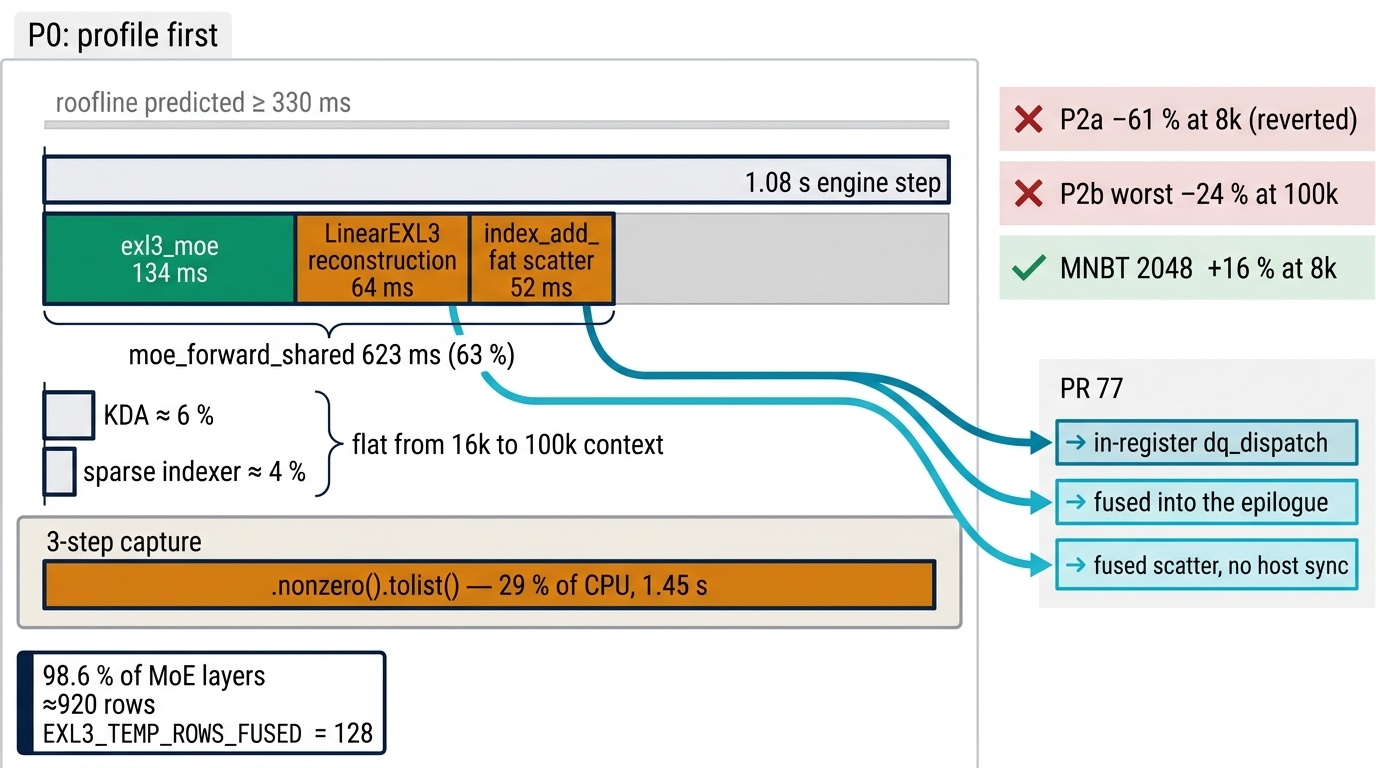
\includegraphics[width=\textwidth]{figures/ch14-p0-profile.png}
\caption{The P0 profile of 2026-08-29 and its consequences. The roofline
predicted a weight-streaming floor of at least 330\,ms; the measured
1.08\,s engine step put \code{moe_forward_shared} at 623\,ms (63\,\%),
inside which \code{exl3_moe} spent 134\,ms, \code{LinearEXL3} reconstruction
64\,ms, and the \code{index_add_} fat scatter 52\,ms, while KDA
($\approx$6\,\%) and the sparse indexer ($\approx$4\,\%) stayed flat from
16k to 100k context. A single \code{.nonzero().tolist()} host sync burned
29\,\% of CPU. Each measured cost maps to what PR~77 did with it; the two
reverted experiments are shown beside the keep.}
\label{fig:qbet-p0}
\end{figure}

\section{PR~77: the E2 kernels}
\label{sec:qbet-e2}

The kernel that specification produced is
\repofile{overlay/exl3_fat_gemm.cu} --- 295
lines of CUDA landed as PR \ghissue{77} in the GLM recipe repository's tracker
(2026-09-01, authored by community contributor plotarmordev). A 50-line
installer compiles it additively into \code{exllamav3_ext}, binding two
new entry points next to \code{exl3_moe}. It replaces the batched tier's
reconstruct-then-\code{hgemm}-then-Hadamard triple with GEMMs that consume
the trellis directly, and it is a compact tour of what a purpose-built
kernel buys over composed primitives: \Cref{fig:qbet-kernel} follows one weight through it.

\begin{itemize}
  \item \textbf{In-register dequantization.} \code{dq_dispatch<4, 1>}
    decodes the K4 MCG trellis words into register fragments per warp ---
    the 4-bit weights are never materialized in memory at all, not even in
    shared memory.
  \item \textbf{Tensor-core MMAs.} The inner loop is \code{ldsm4} loads plus
    \code{ptx_mma_m16n8k16} tensor-core instructions, accumulating in fp32
    across a $128 \times 16 \times 128$ tile.
  \item \textbf{XOR-swizzled shared memory.} Activation tiles are staged
    with a row-derived XOR swizzle matched on the \code{ldsm4} side,
    eliminating shared-memory bank conflicts without padding.
  \item \textbf{The output Hadamard fused into the epilogue.}
    \code{fat_had_ff_128} applies the 128-point output Hadamard transform
    entirely in the epilogue: an in-register 4-point butterfly, two 32-point
    stages built from warp shuffles (\code{shuffle_had_f2x32}), the
    $1/\sqrt{128}$ scale, then the fp16 \code{svh} sign-scales --- the
    separate output-Hadamard pass of the batched tier disappears into the
    GEMM's tail.
  \item \textbf{Scatter mode.} The down-projection entry point
    (\code{exl3_fat_gemm_scatter}) writes
    \code{out[token_idx[row] * N + n] += value * route_weight[row]},
    fusing the per-token route-weight multiply \emph{and} the token scatter
    into the kernel --- with a plain non-atomic \code{+=}. The race-freedom
    argument is a code comment worth quoting: ``One route per token reaches
    a given expert, and expert launches share this stream, so this
    accumulation is race-free.'' Within one expert each token appears once;
    across experts, launches serialize on the same CUDA stream. Correctness
    by scheduling invariant, not by atomics.
\end{itemize}

\begin{figure}[htbp]
\centering
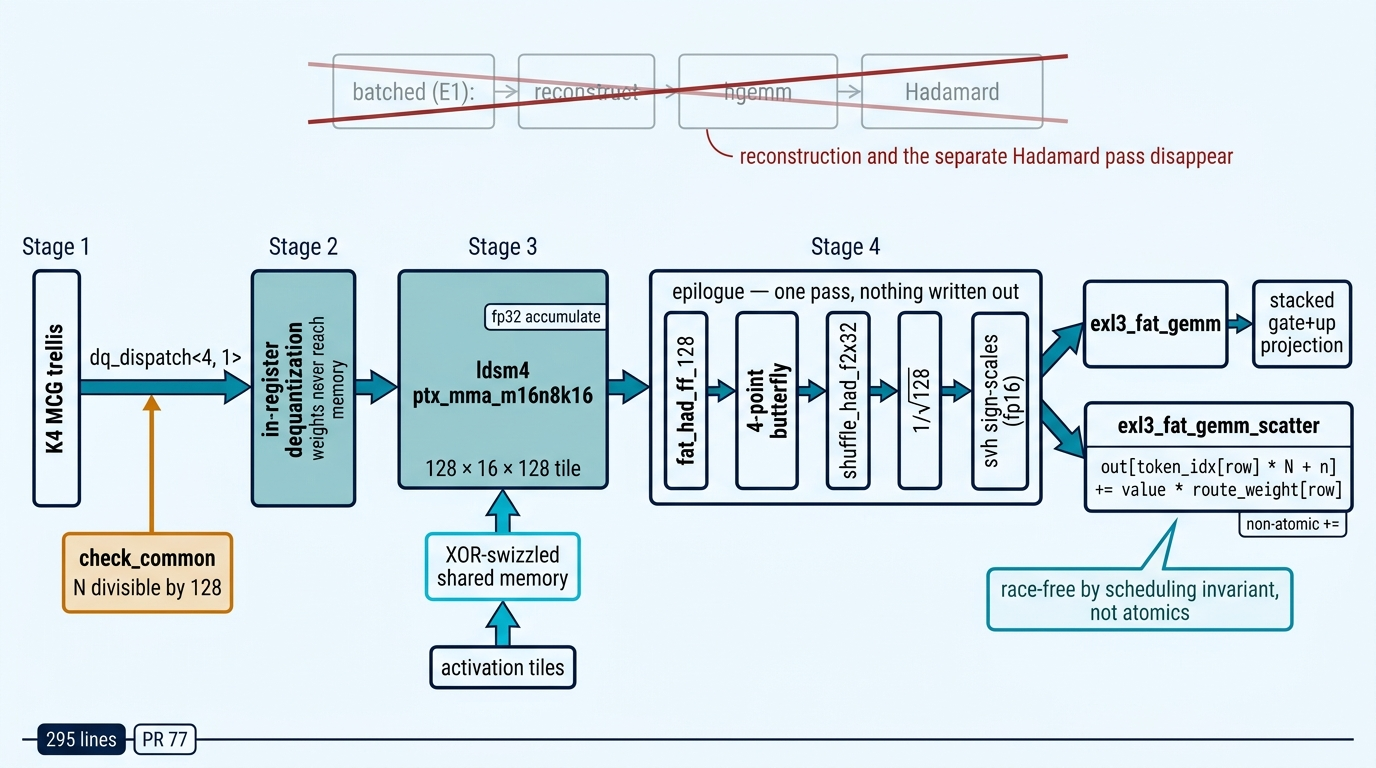
\includegraphics[width=\textwidth]{figures/ch14-e2-kernel-pipeline.png}
\caption{One pass through \repofile{overlay/exl3_fat_gemm.cu}. A K4 MCG
trellis word is decoded into register fragments by \code{dq_dispatch<4, 1>},
multiplied on tensor cores via \code{ldsm4} plus \code{ptx_mma_m16n8k16}
over a $128 \times 16 \times 128$ tile with fp32 accumulation, and finished
inside the epilogue --- Hadamard transform, sign-scales, route weight, and
in scatter mode the token scatter itself --- before any accumulator reaches
memory. The batched tier's reconstruct-then-\code{hgemm}-then-Hadamard
triple, shown struck through above, disappears entirely: the gain is not a
faster GEMM but the removal of the work between GEMMs.}
\label{fig:qbet-kernel}
\end{figure}

Read together the five are one pipeline rather than five separate tricks: a
weight leaves the trellis into registers, is multiplied on tensor cores, and
is finished --- transform, sign-scales, route weight, scatter --- before any
accumulator reaches memory. That is why the gain measured below is not a
faster GEMM but the disappearance of the work that used to happen between
GEMMs.

Guard rails are as characteristic as the fast path: \code{check_common}
rejects anything but K4 MCG tensors, wrong dtypes, non-contiguous inputs,
or an N not divisible by 128 --- the kernel refuses inputs it was not built
for rather than computing something plausible.

The measurement met the repository's own promotion bar: a controlled sequence (E2
on $\to$ legacy off $\to$ E2 on at MNBT 2048) with five unique-salt cold
samples per rung per boot, all 45 observations passing the cold gate with
complete separation. An independent second 2$\times$~DGX Spark kit
reproduced $+21.0$\,\% at 100K and $+20.4$\,\% at 300K.
\Cref{tab:qbet-e2} shows the pooled result that made E2 the production
prefill path (decode is unchanged --- decode batches never exceed the
128-row thin path).

\begin{table}[htbp]
\centering\small
\caption{PR~77 E2 fat-expert kernel: fully uncached prefill, MNBT 2048, five
unique-salt cold samples per rung per boot, 2026-09-01. Reproduced on an
independent second kit ($+21.0$\,\% at 100K, $+20.4$\,\% at 300K).}
\label{tab:qbet-e2}
\begin{tabular}{lrrr}
\toprule
Fully uncached rung & Legacy mean (\tokspersec{}) & PR~77 pooled mean (\tokspersec{}) & Gain \\
\midrule
$\approx$8K   & 941.04  & 1132.32 & $+20.33$\,\% \\
$\approx$100K & 1023.20 & 1241.71 & $+21.36$\,\% \\
$\approx$300K & 995.05  & 1201.02 & $+20.70$\,\% \\
\bottomrule
\end{tabular}
\end{table}

\section{The diagnostics contract}
\label{sec:qbet-diag}

A tier ladder resolved at load, degradations with recorded reasons, kernels
that may or may not be present in a given image --- none of it is auditable
without instrumentation. The E2 work shipped its instrumentation as a
versioned contract rather than ad-hoc logging. Its governing design
requirement is one most diagnostics surfaces never state: \emph{a stale
diagnostic that flatters the system is worse than no diagnostic}.

Two details enforce it. The counter reset
(\code{reset_exl3_fat_diag_counters()}) zeroes the runtime counters but
restarts the scratch-byte counters from the resident cache, so a windowed
read around exactly one cold request still reports honest byte counts
instead of pretending the persistent scratch is free. And the per-layer
labels (\code{_exl3_last_fat_fallback}, \code{_exl3_last_fat_reason},
\code{_exl3_last_apply}) are reset on \emph{every call}, so a
\code{"kernel"} label left over from an earlier prefill --- in the file's
words --- ``cannot masquerade through later decode/thin/row-tile calls.''

The surface those details protect is \code{_EXL3_FAT_DIAG}, a module-level
dict whose key set \emph{is} the API. \code{EXL3_FAT_DIAG_SCHEMA=1}
versions a fixed set of \textbf{32 keys}: load-time facts recording what
was resolved (configured versus effective tier and the degradation reason,
shared-SUH state, symbol availability, CUDA capability, TP rank), and
monotonic runtime counters recording what actually ran --- ``the ground
truth'' in the file's words. The stated rule is that the key set and the
schema number are extended only together, so an external monitor can parse
the output without scraping free-form text.

The whole snapshot renders as one greppable log line, emitted at load (as a
WARNING if the effective tier degraded from the configured one), again
whenever the resolved tier changes between layers, and every 42 layer-stat
records. The cadence is not arbitrary: GLM-5.3-Flash runs 42 routed-MoE
layers per engine step, so each line is exactly one step.
Chapter~\ref{ch:measurement}'s lesson that
instruments deserve regression tests reappears here as: instruments deserve
schemas.

\FloatBarrier

The 4-bit checkpoint stopped being a file on the Hub several sections ago.
What it actually is, on this kit, is a bundle of obligations: a pinned
mirror and a shard count that turn its bytes into an invariant, a KLD panel
that turns its quality into a number, an attention geometry the engine
cannot load until arithmetic reshapes the request, and a 1{,}623-line
backend plus 295 lines of CUDA that make its weights multipliable at all.
The vendor's paved path was never a convenience --- it is the accumulated
discharge of exactly those obligations, and stepping off it means signing
for them yourself, in code, with receipts.

\section*{Takeaways}

\begin{itemize}
  \item Part~II inverts Part~I's bet: the same 2$\times$~GB10 TP=2 kit, but
    a community 4-bpw EXL3 quant that must carry its own quality evidence,
    kernels, and supply chain --- and that supply chain is engineering, not
    a URL. A revision-pinned, byte-identical mirror and a 120-shard
    completeness gate make ``the weights are present'' a checked invariant.
  \item The KLD panel is the bet's receipt: 4\,bpw EXL3 at 0.024555 nats
    statistically ties official FP8's 0.024629 at 54\,\% of the bytes
    (176 vs.\ 328\,GB). The same panel, scoring NVFP4 at 0.060535, is why
    NVFP4 weights and \code{--moe-backend marlin} are banned outright.
  \item When the kernel zoo lacks your geometry, buy an existing kernel
    with memory: zero-padding the 512-dim NoPE latent into the 576-wide
    GLM\_NSA record is mathematically exact at $\approx$24\,\% more DSA KV,
    and the 2051-candidate squeeze discards the four candidates the indexer
    itself ranked least relevant rather than the causal tail no later pool
    expansion could recover.
  \item Degradation is legitimate, mismatch is fatal: a checkpoint that
    does not share gate/up SUH steps the fat-expert ladder down with a
    recorded reason; an image missing a symbol the operator explicitly
    enabled fails the boot instead of becoming a silent no-op.
  \item Profile before building: P0 overturned the roofline, two published
    reverts became PR \ghissue{77}'s specification, and the E2 kernels
    shipped a reproduced $+20$\,\% of uncached prefill behind a versioned
    32-key diagnostics schema.
\end{itemize}

\chaptertransition{Every byte this backend saves is still a byte the decode
step has to stream, and the only way to stop paying for a weight stream is
to stop taking the step --- which is precisely what the drafter riding on
top of this quant exists to do. DFlash2 is a separate $\approx$2.3\,GiB
model run at $k{=}7$, and it bills for itself in a seven-component
acceptance vector on every step: 0.98 sagging to 0.83 on structured output,
0.75 collapsing to 0.06 on prose --- two fingerprints so unalike they amount
to two serving machines inside one serve. There is a third shape, and when
bring-up produced it --- position~0 alive above six dead positions --- it
named a one-line cause that took no profiler, kernel trace, or bisection
to find.}
